\documentclass{BachelorThesis}
\BTsetup{
    info={
        title={XXXXX{\textcolor{red}{(论文题目,楷体一号,居中)}}},
        author={XX},
        studentnumber={XXXXXXXXXX},
        major={XXXX},
        college={物理科学与技术学院},
        supervisor={XXX}
    }
}

\begin{document}
\maketitle

\newpage

\pagenumbering{arabic} %设置阿拉伯数字页码
\tableofcontents

\thispagestyle{empty}

\newpage
\pagestyle{fancy}
\fancyhf{}
\fancyhead[C]{\zihao{5} \songti 武\quad 汉\quad 大\quad 学\quad 本\quad 科\quad 毕\quad 业\quad 论\quad 文\quad ( \quad 设\quad 计 \quad )}
\fancyfoot[C]{\zihao{5} \songti \thepage }
\renewcommand{\headrulewidth}{1pt}
\setcounter{page}{1}

\section{绪论}
\zhlipsum[3] 

这是脚注内容\footnote{这是脚注内容}

这是脚注内容\footnote{这是第二个脚注内容}
\subsection{节标题}
\zhlipsum[4]
\subsubsection{条标题1}
\zhlipsum[1-2]
\subsubsection{条标题2}
\zhlipsum[1-2]

\clearpage

\section{第二章}
\subsection{节标题}
\zhlipsum[2]
\subsubsection{条标题1}
\zhlipsum[6]
\subsubsection{条标题2}
\zhlipsum[7]

测试图片插入:
\begin{figure}[htbp]
  \centering
  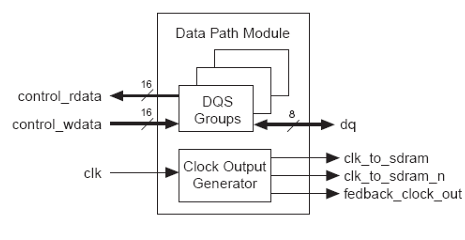
\includegraphics[width=0.5\textwidth]{Figure/数据通道模块内部结构.png}
  \caption{这是一张示例图片}
  \label{fig:example-image}
\end{figure}

测试引用图片:\fref{fig:example-image}

测试表格:
\begin{table}[htbp]
  \centering
%   \zihao{5}
  \normalsize
  \caption{这是一张示例表格}
  \begin{tabular}{m{0.35\textwidth} m{0.35\textwidth} m{0.15\textwidth}}
    \toprule[2pt]
    表头1 & 表头2 & 表头3 \\
    \midrule
    内容1 & 内容2 & 内容3 \\
    内容4 & 内容5 & 内容6 \\
    内容7 & 内容8 & 内容9 \\
    \cline{2-3}
    内容10 & 内容11 & 内容12 \\
    \bottomrule[2pt]
  \end{tabular}
  \label{tab:example-table}
\end{table}

测试引用表格:\tref{tab:example-table}

长表测试:
{\normalsize\begin{longtable}{m{0.3\textwidth}<{\centering}|m{0.7\textwidth}<{\centering}}
  \caption{试验Longtable的四个命令}
  \label{tab:long-table} \\
  \toprule[2pt]
  表头1 & 表头2 \\
  \midrule[1pt]
  \endfirsthead
  %
  \multicolumn{2}{r}{(续表\ref{tab:long-table})}\\
  \toprule[2pt]
  \endhead
  %
  \midrule[1pt]
  \endfoot
  %
  \bottomrule[2pt]
  \endlastfoot
  %
  1  & a \\
  2  & b \\
  3  & c \\
  4  & d \\
  5  & e \\
  6  & f \\
  7  & g \\
  8  & h \\
  9  & i \\
  10 & j \\
  11 & k \\
  12 & l \\
  13 & m \\
  14 & n \\
  15 & o \\
  16 & p \\
  17 & q \\
  18 & r \\
  19 & s \\
  20 & t \\
  21 & u \\
  22 & v \\
  23 & w \\
  24 & x \\
  25 & y \\
  26 & z \\
  27 & A \\
  28 & B \\
  29 & C \\
  30 & D \\
  31 & E \\
  32 & F \\
  33 & G \\
  34 & H \\
  35 & I \\
  36 & J \\
  37 & K \\
  38 & L \\
  39 & M \\
  40 & N \\
  41 & O \\
  42 & P \\
  43 & Q \\
  44 & R \\
  45 & S \\
  46 & T \\
  47 & U \\
  48 & V \\
  49 & W \\
  50 & X \\
  51 & Y \\
  52 & Z \\
\end{longtable}}

测试引用长表:\tref{tab:long-table}


测试公式:
\begin{equation}
  \label{eq:example-equation}
  E = mc^2
\end{equation}

测试引用公式:\eqref{eq:example-equation}


测试bibliography:\cite{zhang2023effects},\cite{author2023example}
\clearpage
\section{结论}

\zhlipsum[1-2]

\clearpage
\addcontentsline{toc}{section}{参考文献}%将摘要放进目录
\bibliographystyle{gbt7714-2005-whu-numerical}
\bibliography{reference}
\clearpage
\section*{致\quad 谢}
\addcontentsline{toc}{section}{致谢}
\zhlipsum[1-2]
\clearpage
\section*{附录}
\addcontentsline{toc}{section}{附录}
\zhlipsum[1-2]
\end{document}